\documentclass[twoside]{book}

% Packages required by doxygen
\usepackage{calc}
\usepackage{doxygen}
\usepackage{graphicx}
\usepackage[utf8]{inputenc}
\usepackage{makeidx}
\usepackage{multicol}
\usepackage{multirow}
\usepackage{textcomp}
\usepackage[table]{xcolor}

% Font selection
\usepackage[T1]{fontenc}
\usepackage{mathptmx}
\usepackage[scaled=.90]{helvet}
\usepackage{courier}
\usepackage{amssymb}
\usepackage{sectsty}
\renewcommand{\familydefault}{\sfdefault}
\allsectionsfont{%
  \fontseries{bc}\selectfont%
  \color{darkgray}%
}
\renewcommand{\DoxyLabelFont}{%
  \fontseries{bc}\selectfont%
  \color{darkgray}%
}

% Page & text layout
\usepackage{geometry}
\geometry{%
  a4paper,%
  top=2.5cm,%
  bottom=2.5cm,%
  left=2.5cm,%
  right=2.5cm%
}
\tolerance=750
\hfuzz=15pt
\hbadness=750
\setlength{\emergencystretch}{15pt}
\setlength{\parindent}{0cm}
\setlength{\parskip}{0.2cm}
\makeatletter
\renewcommand{\paragraph}{%
  \@startsection{paragraph}{4}{0ex}{-1.0ex}{1.0ex}{%
    \normalfont\normalsize\bfseries\SS@parafont%
  }%
}
\renewcommand{\subparagraph}{%
  \@startsection{subparagraph}{5}{0ex}{-1.0ex}{1.0ex}{%
    \normalfont\normalsize\bfseries\SS@subparafont%
  }%
}
\makeatother

% Headers & footers
\usepackage{fancyhdr}
\pagestyle{fancyplain}
\fancyhead[LE]{\fancyplain{}{\bfseries\thepage}}
\fancyhead[CE]{\fancyplain{}{}}
\fancyhead[RE]{\fancyplain{}{\bfseries\leftmark}}
\fancyhead[LO]{\fancyplain{}{\bfseries\rightmark}}
\fancyhead[CO]{\fancyplain{}{}}
\fancyhead[RO]{\fancyplain{}{\bfseries\thepage}}
\fancyfoot[LE]{\fancyplain{}{}}
\fancyfoot[CE]{\fancyplain{}{}}
\fancyfoot[RE]{\fancyplain{}{\bfseries\scriptsize Generated on Wed May 20 2015 23\-:05\-:28 for Midgard Map\-Maker by Doxygen }}
\fancyfoot[LO]{\fancyplain{}{\bfseries\scriptsize Generated on Wed May 20 2015 23\-:05\-:28 for Midgard Map\-Maker by Doxygen }}
\fancyfoot[CO]{\fancyplain{}{}}
\fancyfoot[RO]{\fancyplain{}{}}
\renewcommand{\footrulewidth}{0.4pt}
\renewcommand{\chaptermark}[1]{%
  \markboth{#1}{}%
}
\renewcommand{\sectionmark}[1]{%
  \markright{\thesection\ #1}%
}

% Indices & bibliography
\usepackage{natbib}
\usepackage[titles]{tocloft}
\setcounter{tocdepth}{3}
\setcounter{secnumdepth}{5}
\makeindex

% Hyperlinks (required, but should be loaded last)
\usepackage{ifpdf}
\ifpdf
  \usepackage[pdftex,pagebackref=true]{hyperref}
\else
  \usepackage[ps2pdf,pagebackref=true]{hyperref}
\fi
\hypersetup{%
  colorlinks=true,%
  linkcolor=blue,%
  citecolor=blue,%
  unicode%
}

% Custom commands
\newcommand{\clearemptydoublepage}{%
  \newpage{\pagestyle{empty}\cleardoublepage}%
}


%===== C O N T E N T S =====

\begin{document}

% Titlepage & ToC
\hypersetup{pageanchor=false}
\pagenumbering{roman}
\begin{titlepage}
\vspace*{7cm}
\begin{center}%
{\Large Midgard Map\-Maker \\[1ex]\large Final Realease }\\
\vspace*{1cm}
{\large Generated by Doxygen 1.8.6}\\
\vspace*{0.5cm}
{\small Wed May 20 2015 23:05:28}\\
\end{center}
\end{titlepage}
\clearemptydoublepage
\tableofcontents
\clearemptydoublepage
\pagenumbering{arabic}
\hypersetup{pageanchor=true}

%--- Begin generated contents ---
\chapter{Midgar-\/\-Map-\/\-Maker}
\label{md__home_cristianfernando__documentos_git__midgard_map_maker__r_e_a_d_m_e}
\hypertarget{md__home_cristianfernando__documentos_git__midgard_map_maker__r_e_a_d_m_e}{}
\input{md__home_cristianfernando__documentos_git__midgard_map_maker__r_e_a_d_m_e}
\chapter{Hierarchical Index}
\section{Class Hierarchy}
This inheritance list is sorted roughly, but not completely, alphabetically\-:\begin{DoxyCompactList}
\item Q\-Dialog\begin{DoxyCompactList}
\item \contentsline{section}{Map\-Name}{\pageref{class_map_name}}{}
\item \contentsline{section}{Map\-Size}{\pageref{class_map_size}}{}
\end{DoxyCompactList}
\item Q\-Main\-Window\begin{DoxyCompactList}
\item \contentsline{section}{Map\-Maker}{\pageref{class_map_maker}}{}
\end{DoxyCompactList}
\item Q\-Thread\begin{DoxyCompactList}
\item \contentsline{section}{Updater}{\pageref{class_updater}}{}
\end{DoxyCompactList}
\item Q\-Widget\begin{DoxyCompactList}
\item \contentsline{section}{Terrain\-Painter}{\pageref{class_terrain_painter}}{}
\end{DoxyCompactList}
\end{DoxyCompactList}

\chapter{Class Index}
\section{Class List}
Here are the classes, structs, unions and interfaces with brief descriptions\-:\begin{DoxyCompactList}
\item\contentsline{section}{\hyperlink{class_map_maker}{Map\-Maker} \\*Clase \hyperlink{class_map_maker}{Map\-Maker} es la clase que actua con el usuario, es una ventana con algunos botones con los que se puede editar un mapa del programa Midgard, el proyecto Midgard se puede encontrar en el siguiente hipervinculo \hyperlink{}{https\-://github.\-com/\-Programmer-\/\-C\-E/\-Midgard-\/\-Project}}{\pageref{class_map_maker}}{}
\item\contentsline{section}{\hyperlink{class_map_name}{Map\-Name} \\*Es un dialogo que se encarga de obtener el nombre del mapa esto es un nombre representativo para el controlardor servidores en el proyecto Midgard, este dialogo es arrojado cuando se guarda un archivo por primera vez }{\pageref{class_map_name}}{}
\item\contentsline{section}{\hyperlink{class_map_size}{Map\-Size} \\*Es un dialogo que se encarga de obtener el tamanio del nuevo mapa a crear }{\pageref{class_map_size}}{}
\item\contentsline{section}{\hyperlink{class_terrain_painter}{Terrain\-Painter} \\*Clase \hyperlink{class_terrain_painter}{Terrain\-Painter}, se encarga de pintar el mapa y gestionarlo asi como de guardarlo o cargar un mapa de un disco rigido }{\pageref{class_terrain_painter}}{}
\item\contentsline{section}{\hyperlink{class_updater}{Updater} }{\pageref{class_updater}}{}
\end{DoxyCompactList}

\chapter{Class Documentation}
\hypertarget{class_map_maker}{\section{Map\-Maker Class Reference}
\label{class_map_maker}\index{Map\-Maker@{Map\-Maker}}
}


Clase \hyperlink{class_map_maker}{Map\-Maker} es la clase que actua con el usuario, es una ventana con algunos botones con los que se puede editar un mapa del programa Midgard, el proyecto Midgard se puede encontrar en el siguiente hipervinculo \hyperlink{}{https\-://github.\-com/\-Programmer-\/\-C\-E/\-Midgard-\/\-Project.} 




{\ttfamily \#include $<$mapmaker.\-h$>$}

Inheritance diagram for Map\-Maker\-:\begin{figure}[H]
\begin{center}
\leavevmode
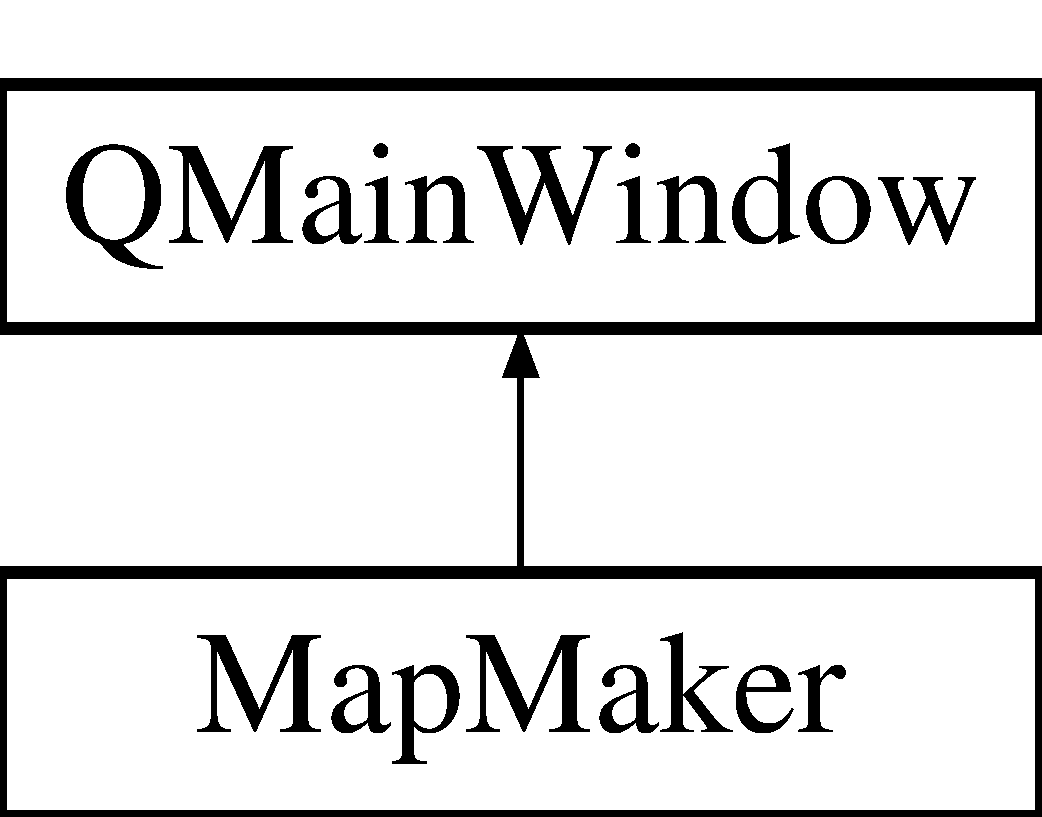
\includegraphics[height=2.000000cm]{class_map_maker}
\end{center}
\end{figure}
\subsection*{Public Slots}
\begin{DoxyCompactItemize}
\item 
\hypertarget{class_map_maker_a9947055f482f31c770769b952e53bf67}{void \hyperlink{class_map_maker_a9947055f482f31c770769b952e53bf67}{set\-Active\-Tile\-Set} ()}\label{class_map_maker_a9947055f482f31c770769b952e53bf67}

\begin{DoxyCompactList}\small\item\em Setea el tipo de celda a insertar depende de las opciones de radiobutton con las etiquetas tierra y bosque. \end{DoxyCompactList}\item 
\hypertarget{class_map_maker_a9a8bba5beafacbb6432fc1d7013548fe}{void \hyperlink{class_map_maker_a9a8bba5beafacbb6432fc1d7013548fe}{change\-Mouse\-Action} ()}\label{class_map_maker_a9a8bba5beafacbb6432fc1d7013548fe}

\begin{DoxyCompactList}\small\item\em Es la accion del mouse borra los elementos de bosque en las celdas del mapa. \end{DoxyCompactList}\item 
\hypertarget{class_map_maker_a8e4f57b9449a8655c3edf8dd3f5c219d}{void \hyperlink{class_map_maker_a8e4f57b9449a8655c3edf8dd3f5c219d}{save\-Data} ()}\label{class_map_maker_a8e4f57b9449a8655c3edf8dd3f5c219d}

\begin{DoxyCompactList}\small\item\em Arroja una ventana que solicita el nombre del mapa con la cual se quiere representar, luego arroja otra ventana de buscador de archivos con el cual se solicita la direccion a guardar del mapa si se selecciono una direccion de guardado se procede a guardar un xml en la direccion solicitada. No es necesario colocar la extension del archivo ya que esta se coloca automaticamente. El archivo guardado es un xml aun asi si el usuario no lo desea. \end{DoxyCompactList}\item 
\hypertarget{class_map_maker_a6460a1ae322e8484240ddde66bc57144}{void \hyperlink{class_map_maker_a6460a1ae322e8484240ddde66bc57144}{simple\-Save\-Data} ()}\label{class_map_maker_a6460a1ae322e8484240ddde66bc57144}

\begin{DoxyCompactList}\small\item\em Se encarga de guardar los cambios en el mismo archivo, se recomienda que se use el shortcut Alt+\-G. \end{DoxyCompactList}\item 
void \hyperlink{class_map_maker_a79fd5a327db129f3876895aa1ef9dc24}{create\-New\-Map} ()
\begin{DoxyCompactList}\small\item\em Se encarga de crear un nuevo mapa de un tamanio seleccionado. \end{DoxyCompactList}\item 
\hypertarget{class_map_maker_a453e645083e5444d39ae6d52f6829e7d}{void \hyperlink{class_map_maker_a453e645083e5444d39ae6d52f6829e7d}{load\-Data} ()}\label{class_map_maker_a453e645083e5444d39ae6d52f6829e7d}

\begin{DoxyCompactList}\small\item\em Se encarga de abrir un archivo xml si este sigue con el standar definido en el xml schema llamado esquema.\-xsd entonces el archivo es cargado a memoria de lo contrario el archivo no se abre y se arroja un dialogo con el respectivo texto. \end{DoxyCompactList}\end{DoxyCompactItemize}
\subsection*{Public Member Functions}
\begin{DoxyCompactItemize}
\item 
\hyperlink{class_map_maker_a45cd33bb40e93ad7c96171240e87a7bd}{Map\-Maker} (Q\-Widget $\ast$parent=0)
\begin{DoxyCompactList}\small\item\em Es el constructor inicializa un mapa por defecto de tamanio 64 celdas por 64 celdas. \end{DoxyCompactList}\item 
bool \hyperlink{class_map_maker_ac56883ea2ed2c8d85824ba94f960a504}{get\-Mouse\-Action} ()
\begin{DoxyCompactList}\small\item\em Obtiene la accion del mouse. \end{DoxyCompactList}\item 
bool \hyperlink{class_map_maker_a35b3c5bae988e2dce39926ef6240ab10}{get\-Tile\-Set\-Active} ()
\begin{DoxyCompactList}\small\item\em Retorna la bandera que indica que tipo de elemento desea insertarse. \end{DoxyCompactList}\item 
\hyperlink{class_terrain_painter}{Terrain\-Painter} $\ast$ \hyperlink{class_map_maker_a6c01882f3158db7f771f12460bff31b1}{get\-Terrain\-Painter} ()
\begin{DoxyCompactList}\small\item\em Obtiene objeto que se encarga de pintar el mapa. \end{DoxyCompactList}\item 
\hypertarget{class_map_maker_a270d6592f31c8026c809501ff4f2c2b9}{\hyperlink{class_map_maker_a270d6592f31c8026c809501ff4f2c2b9}{$\sim$\-Map\-Maker} ()}\label{class_map_maker_a270d6592f31c8026c809501ff4f2c2b9}

\begin{DoxyCompactList}\small\item\em Es el destructor y liberador de memoria. \end{DoxyCompactList}\end{DoxyCompactItemize}
\subsection*{Protected Member Functions}
\begin{DoxyCompactItemize}
\item 
void \hyperlink{class_map_maker_a1dced69406f01f92ae06b7965c0b90bc}{close\-Event} (Q\-Close\-Event $\ast$p\-Close\-Event)
\begin{DoxyCompactList}\small\item\em Es el evento que se encarga de cerrar el la ventana correctamente. \end{DoxyCompactList}\end{DoxyCompactItemize}


\subsection{Detailed Description}
Clase \hyperlink{class_map_maker}{Map\-Maker} es la clase que actua con el usuario, es una ventana con algunos botones con los que se puede editar un mapa del programa Midgard, el proyecto Midgard se puede encontrar en el siguiente hipervinculo \hyperlink{}{https\-://github.\-com/\-Programmer-\/\-C\-E/\-Midgard-\/\-Project.}

\subsection{Constructor \& Destructor Documentation}
\hypertarget{class_map_maker_a45cd33bb40e93ad7c96171240e87a7bd}{\index{Map\-Maker@{Map\-Maker}!Map\-Maker@{Map\-Maker}}
\index{Map\-Maker@{Map\-Maker}!MapMaker@{Map\-Maker}}
\subsubsection[{Map\-Maker}]{\setlength{\rightskip}{0pt plus 5cm}Map\-Maker\-::\-Map\-Maker (
\begin{DoxyParamCaption}
\item[{Q\-Widget $\ast$}]{parent = {\ttfamily 0}}
\end{DoxyParamCaption}
)\hspace{0.3cm}{\ttfamily [explicit]}}}\label{class_map_maker_a45cd33bb40e93ad7c96171240e87a7bd}


Es el constructor inicializa un mapa por defecto de tamanio 64 celdas por 64 celdas. 


\begin{DoxyParams}{Parameters}
{\em parent} & es el complemtento en el que se ejecutara esta ventana \\
\hline
\end{DoxyParams}


\subsection{Member Function Documentation}
\hypertarget{class_map_maker_a1dced69406f01f92ae06b7965c0b90bc}{\index{Map\-Maker@{Map\-Maker}!close\-Event@{close\-Event}}
\index{close\-Event@{close\-Event}!MapMaker@{Map\-Maker}}
\subsubsection[{close\-Event}]{\setlength{\rightskip}{0pt plus 5cm}void Map\-Maker\-::close\-Event (
\begin{DoxyParamCaption}
\item[{Q\-Close\-Event $\ast$}]{p\-Close\-Event}
\end{DoxyParamCaption}
)\hspace{0.3cm}{\ttfamily [protected]}}}\label{class_map_maker_a1dced69406f01f92ae06b7965c0b90bc}


Es el evento que se encarga de cerrar el la ventana correctamente. 


\begin{DoxyParams}{Parameters}
{\em p\-Close\-Event} & Es el evento de cierre \\
\hline
\end{DoxyParams}
\hypertarget{class_map_maker_a79fd5a327db129f3876895aa1ef9dc24}{\index{Map\-Maker@{Map\-Maker}!create\-New\-Map@{create\-New\-Map}}
\index{create\-New\-Map@{create\-New\-Map}!MapMaker@{Map\-Maker}}
\subsubsection[{create\-New\-Map}]{\setlength{\rightskip}{0pt plus 5cm}void Map\-Maker\-::create\-New\-Map (
\begin{DoxyParamCaption}
{}
\end{DoxyParamCaption}
)\hspace{0.3cm}{\ttfamily [slot]}}}\label{class_map_maker_a79fd5a327db129f3876895aa1ef9dc24}


Se encarga de crear un nuevo mapa de un tamanio seleccionado. 

ui-\/$>$scroll\-Area-\/$>$set\-Maximum\-Size(ui-\/$>$widget-\/$>$minimum\-Size()); set\-Maximum\-Size(ui-\/$>$scroll\-Area\-Widget\-Contents-\/$>$minimum\-Size());\hypertarget{class_map_maker_ac56883ea2ed2c8d85824ba94f960a504}{\index{Map\-Maker@{Map\-Maker}!get\-Mouse\-Action@{get\-Mouse\-Action}}
\index{get\-Mouse\-Action@{get\-Mouse\-Action}!MapMaker@{Map\-Maker}}
\subsubsection[{get\-Mouse\-Action}]{\setlength{\rightskip}{0pt plus 5cm}bool Map\-Maker\-::get\-Mouse\-Action (
\begin{DoxyParamCaption}
{}
\end{DoxyParamCaption}
)}}\label{class_map_maker_ac56883ea2ed2c8d85824ba94f960a504}


Obtiene la accion del mouse. 

\begin{DoxyReturn}{Returns}
true si la accion es agregar, false si la accion es quitar 
\end{DoxyReturn}
\hypertarget{class_map_maker_a6c01882f3158db7f771f12460bff31b1}{\index{Map\-Maker@{Map\-Maker}!get\-Terrain\-Painter@{get\-Terrain\-Painter}}
\index{get\-Terrain\-Painter@{get\-Terrain\-Painter}!MapMaker@{Map\-Maker}}
\subsubsection[{get\-Terrain\-Painter}]{\setlength{\rightskip}{0pt plus 5cm}{\bf Terrain\-Painter} $\ast$ Map\-Maker\-::get\-Terrain\-Painter (
\begin{DoxyParamCaption}
{}
\end{DoxyParamCaption}
)}}\label{class_map_maker_a6c01882f3158db7f771f12460bff31b1}


Obtiene objeto que se encarga de pintar el mapa. 

\begin{DoxyReturn}{Returns}
\hyperlink{class_terrain_painter}{Terrain\-Painter} es el objeto que se encaga de pintar el mapa 
\end{DoxyReturn}
\hypertarget{class_map_maker_a35b3c5bae988e2dce39926ef6240ab10}{\index{Map\-Maker@{Map\-Maker}!get\-Tile\-Set\-Active@{get\-Tile\-Set\-Active}}
\index{get\-Tile\-Set\-Active@{get\-Tile\-Set\-Active}!MapMaker@{Map\-Maker}}
\subsubsection[{get\-Tile\-Set\-Active}]{\setlength{\rightskip}{0pt plus 5cm}bool Map\-Maker\-::get\-Tile\-Set\-Active (
\begin{DoxyParamCaption}
{}
\end{DoxyParamCaption}
)}}\label{class_map_maker_a35b3c5bae988e2dce39926ef6240ab10}


Retorna la bandera que indica que tipo de elemento desea insertarse. 

\begin{DoxyReturn}{Returns}
true si se desea insertar bosque, que es un obstaculo, y false si se desea insertar tierra o terreno que no es un obstaculo 
\end{DoxyReturn}


The documentation for this class was generated from the following files\-:\begin{DoxyCompactItemize}
\item 
/home/cristianfernando/\-Documentos/git/\-Midgard\-Map\-Maker/mapmaker.\-h\item 
/home/cristianfernando/\-Documentos/git/\-Midgard\-Map\-Maker/mapmaker.\-cpp\end{DoxyCompactItemize}

\hypertarget{class_map_name}{\section{Map\-Name Class Reference}
\label{class_map_name}\index{Map\-Name@{Map\-Name}}
}


Es un dialogo que se encarga de obtener el nombre del mapa esto es un nombre representativo para el controlardor servidores en el proyecto Midgard, este dialogo es arrojado cuando se guarda un archivo por primera vez.  




{\ttfamily \#include $<$mapname.\-h$>$}

Inheritance diagram for Map\-Name\-:\begin{figure}[H]
\begin{center}
\leavevmode
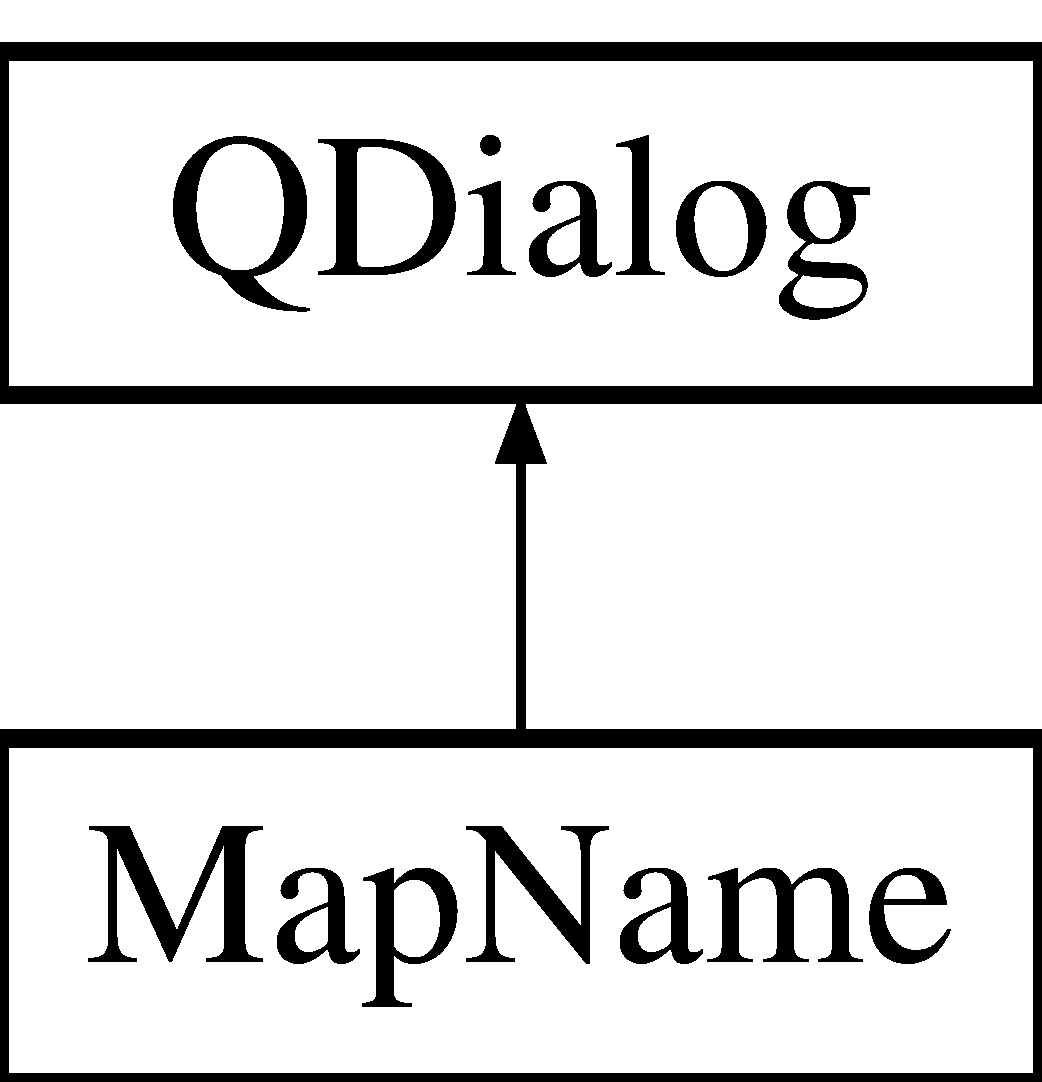
\includegraphics[height=2.000000cm]{class_map_name}
\end{center}
\end{figure}
\subsection*{Public Slots}
\begin{DoxyCompactItemize}
\item 
\hypertarget{class_map_name_a2d10ccd3853afeb9f30c2336eb138e04}{void \hyperlink{class_map_name_a2d10ccd3853afeb9f30c2336eb138e04}{accept} ()}\label{class_map_name_a2d10ccd3853afeb9f30c2336eb138e04}

\begin{DoxyCompactList}\small\item\em se sobrescribe si no existe un nombre representativo para el mapa entonces se arroja un dialogo con un mensaje indicando que debe insertarse un nombre, se acepta el dialogo si se inserta un nombre \end{DoxyCompactList}\item 
\hypertarget{class_map_name_afaa02200b9a312c6b7865fc19e6ec52f}{void \hyperlink{class_map_name_afaa02200b9a312c6b7865fc19e6ec52f}{reject} ()}\label{class_map_name_afaa02200b9a312c6b7865fc19e6ec52f}

\begin{DoxyCompactList}\small\item\em no hace nada pues no se puede rechazar el dialogo, la unica forma de que el dialogo se \char`\"{}quite\char`\"{} es aceptandolo \end{DoxyCompactList}\end{DoxyCompactItemize}
\subsection*{Public Member Functions}
\begin{DoxyCompactItemize}
\item 
\hyperlink{class_map_name_a180dde809a405229689bfb7d84145701}{Map\-Name} (Q\-Widget $\ast$parent=0)
\begin{DoxyCompactList}\small\item\em Es el constructor por defecto. \end{DoxyCompactList}\item 
Q\-String \hyperlink{class_map_name_a0c7db97256abcc52b7e7321d0c86c67d}{name\-Of\-Map} () const 
\begin{DoxyCompactList}\small\item\em Retorna el nombre representativo del mapa. \end{DoxyCompactList}\item 
void \hyperlink{class_map_name_a74a823e51c1e47ee0e76abec43a3fd05}{set\-Name\-Of\-Map} (Q\-String p\-Name)
\begin{DoxyCompactList}\small\item\em Setea el nombre del mapa. \end{DoxyCompactList}\item 
\hypertarget{class_map_name_a341bb66bf5d06a9ff0a41ffa289893bb}{\hyperlink{class_map_name_a341bb66bf5d06a9ff0a41ffa289893bb}{$\sim$\-Map\-Name} ()}\label{class_map_name_a341bb66bf5d06a9ff0a41ffa289893bb}

\begin{DoxyCompactList}\small\item\em Es el destructor, limpia la memoria. \end{DoxyCompactList}\end{DoxyCompactItemize}


\subsection{Detailed Description}
Es un dialogo que se encarga de obtener el nombre del mapa esto es un nombre representativo para el controlardor servidores en el proyecto Midgard, este dialogo es arrojado cuando se guarda un archivo por primera vez. 

\subsection{Constructor \& Destructor Documentation}
\hypertarget{class_map_name_a180dde809a405229689bfb7d84145701}{\index{Map\-Name@{Map\-Name}!Map\-Name@{Map\-Name}}
\index{Map\-Name@{Map\-Name}!MapName@{Map\-Name}}
\subsubsection[{Map\-Name}]{\setlength{\rightskip}{0pt plus 5cm}Map\-Name\-::\-Map\-Name (
\begin{DoxyParamCaption}
\item[{Q\-Widget $\ast$}]{parent = {\ttfamily 0}}
\end{DoxyParamCaption}
)\hspace{0.3cm}{\ttfamily [explicit]}}}\label{class_map_name_a180dde809a405229689bfb7d84145701}


Es el constructor por defecto. 


\begin{DoxyParams}{Parameters}
{\em parent} & \\
\hline
\end{DoxyParams}


\subsection{Member Function Documentation}
\hypertarget{class_map_name_a0c7db97256abcc52b7e7321d0c86c67d}{\index{Map\-Name@{Map\-Name}!name\-Of\-Map@{name\-Of\-Map}}
\index{name\-Of\-Map@{name\-Of\-Map}!MapName@{Map\-Name}}
\subsubsection[{name\-Of\-Map}]{\setlength{\rightskip}{0pt plus 5cm}Q\-String Map\-Name\-::name\-Of\-Map (
\begin{DoxyParamCaption}
{}
\end{DoxyParamCaption}
) const}}\label{class_map_name_a0c7db97256abcc52b7e7321d0c86c67d}


Retorna el nombre representativo del mapa. 

\begin{DoxyReturn}{Returns}
el nombre representativo del mapa 
\end{DoxyReturn}
\hypertarget{class_map_name_a74a823e51c1e47ee0e76abec43a3fd05}{\index{Map\-Name@{Map\-Name}!set\-Name\-Of\-Map@{set\-Name\-Of\-Map}}
\index{set\-Name\-Of\-Map@{set\-Name\-Of\-Map}!MapName@{Map\-Name}}
\subsubsection[{set\-Name\-Of\-Map}]{\setlength{\rightskip}{0pt plus 5cm}void Map\-Name\-::set\-Name\-Of\-Map (
\begin{DoxyParamCaption}
\item[{Q\-String}]{p\-Name}
\end{DoxyParamCaption}
)}}\label{class_map_name_a74a823e51c1e47ee0e76abec43a3fd05}


Setea el nombre del mapa. 


\begin{DoxyParams}{Parameters}
{\em p\-Name} & es el nombre a setear \\
\hline
\end{DoxyParams}


The documentation for this class was generated from the following files\-:\begin{DoxyCompactItemize}
\item 
/home/cristianfernando/\-Documentos/git/\-Midgard\-Map\-Maker/mapname.\-h\item 
/home/cristianfernando/\-Documentos/git/\-Midgard\-Map\-Maker/mapname.\-cpp\end{DoxyCompactItemize}

\hypertarget{class_map_size}{\section{Map\-Size Class Reference}
\label{class_map_size}\index{Map\-Size@{Map\-Size}}
}


Es un dialogo que se encarga de obtener el tamanio del nuevo mapa a crear.  




{\ttfamily \#include $<$mapsize.\-h$>$}

Inheritance diagram for Map\-Size\-:\begin{figure}[H]
\begin{center}
\leavevmode
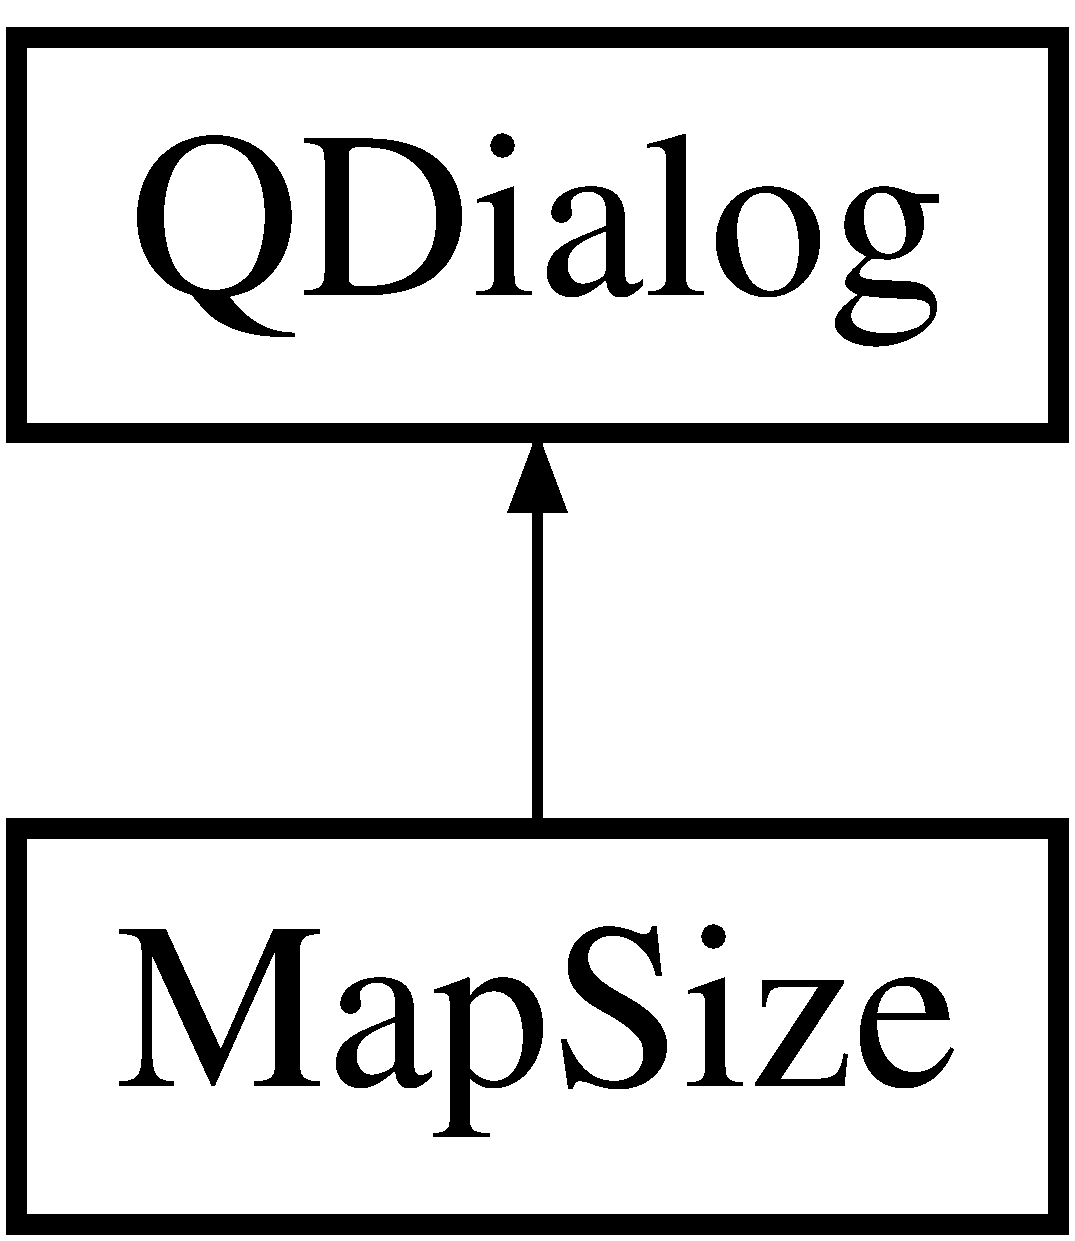
\includegraphics[height=2.000000cm]{class_map_size}
\end{center}
\end{figure}
\subsection*{Public Member Functions}
\begin{DoxyCompactItemize}
\item 
\hyperlink{class_map_size_aaad41b69e09aad8500a60115663abba7}{Map\-Size} (Q\-Widget $\ast$parent=0)
\begin{DoxyCompactList}\small\item\em Es el constructor por defecto. \end{DoxyCompactList}\item 
\hypertarget{class_map_size_a3f200dce80be15b15093469b6b6df3fa}{\hyperlink{class_map_size_a3f200dce80be15b15093469b6b6df3fa}{$\sim$\-Map\-Size} ()}\label{class_map_size_a3f200dce80be15b15093469b6b6df3fa}

\begin{DoxyCompactList}\small\item\em Es el destructor. \end{DoxyCompactList}\item 
int \hyperlink{class_map_size_afb2d611ef961cd31a98c5a8fcbd87341}{get\-Height\-Of\-New\-Map} ()
\begin{DoxyCompactList}\small\item\em Obtiene el tamanio de la altura del mapa, esta altura esta dada en numero de celdas. \end{DoxyCompactList}\item 
int \hyperlink{class_map_size_a9fad6a10e445b1fd4c593cd5c7f98d48}{get\-Width\-Of\-New\-Map} ()
\begin{DoxyCompactList}\small\item\em Obtiene el tamanio de la anchura del mapa, la anchura se da en celdas de mapa. \end{DoxyCompactList}\end{DoxyCompactItemize}


\subsection{Detailed Description}
Es un dialogo que se encarga de obtener el tamanio del nuevo mapa a crear. 

\subsection{Constructor \& Destructor Documentation}
\hypertarget{class_map_size_aaad41b69e09aad8500a60115663abba7}{\index{Map\-Size@{Map\-Size}!Map\-Size@{Map\-Size}}
\index{Map\-Size@{Map\-Size}!MapSize@{Map\-Size}}
\subsubsection[{Map\-Size}]{\setlength{\rightskip}{0pt plus 5cm}Map\-Size\-::\-Map\-Size (
\begin{DoxyParamCaption}
\item[{Q\-Widget $\ast$}]{parent = {\ttfamily 0}}
\end{DoxyParamCaption}
)\hspace{0.3cm}{\ttfamily [explicit]}}}\label{class_map_size_aaad41b69e09aad8500a60115663abba7}


Es el constructor por defecto. 


\begin{DoxyParams}{Parameters}
{\em parent} & \\
\hline
\end{DoxyParams}


\subsection{Member Function Documentation}
\hypertarget{class_map_size_afb2d611ef961cd31a98c5a8fcbd87341}{\index{Map\-Size@{Map\-Size}!get\-Height\-Of\-New\-Map@{get\-Height\-Of\-New\-Map}}
\index{get\-Height\-Of\-New\-Map@{get\-Height\-Of\-New\-Map}!MapSize@{Map\-Size}}
\subsubsection[{get\-Height\-Of\-New\-Map}]{\setlength{\rightskip}{0pt plus 5cm}int Map\-Size\-::get\-Height\-Of\-New\-Map (
\begin{DoxyParamCaption}
{}
\end{DoxyParamCaption}
)}}\label{class_map_size_afb2d611ef961cd31a98c5a8fcbd87341}


Obtiene el tamanio de la altura del mapa, esta altura esta dada en numero de celdas. 

\begin{DoxyReturn}{Returns}
la cantidad de celdas verticalmente 
\end{DoxyReturn}
\hypertarget{class_map_size_a9fad6a10e445b1fd4c593cd5c7f98d48}{\index{Map\-Size@{Map\-Size}!get\-Width\-Of\-New\-Map@{get\-Width\-Of\-New\-Map}}
\index{get\-Width\-Of\-New\-Map@{get\-Width\-Of\-New\-Map}!MapSize@{Map\-Size}}
\subsubsection[{get\-Width\-Of\-New\-Map}]{\setlength{\rightskip}{0pt plus 5cm}int Map\-Size\-::get\-Width\-Of\-New\-Map (
\begin{DoxyParamCaption}
{}
\end{DoxyParamCaption}
)}}\label{class_map_size_a9fad6a10e445b1fd4c593cd5c7f98d48}


Obtiene el tamanio de la anchura del mapa, la anchura se da en celdas de mapa. 

\begin{DoxyReturn}{Returns}
la cantidad de celdas horizontalmente 
\end{DoxyReturn}


The documentation for this class was generated from the following files\-:\begin{DoxyCompactItemize}
\item 
/home/cristianfernando/\-Documentos/git/\-Midgard\-Map\-Maker/mapsize.\-h\item 
/home/cristianfernando/\-Documentos/git/\-Midgard\-Map\-Maker/mapsize.\-cpp\end{DoxyCompactItemize}

\hypertarget{class_terrain_painter}{\section{Terrain\-Painter Class Reference}
\label{class_terrain_painter}\index{Terrain\-Painter@{Terrain\-Painter}}
}


Clase \hyperlink{class_terrain_painter}{Terrain\-Painter}, se encarga de pintar el mapa y gestionarlo asi como de guardarlo o cargar un mapa de un disco rigido.  




{\ttfamily \#include $<$terrainpainter.\-h$>$}

Inheritance diagram for Terrain\-Painter\-:\begin{figure}[H]
\begin{center}
\leavevmode
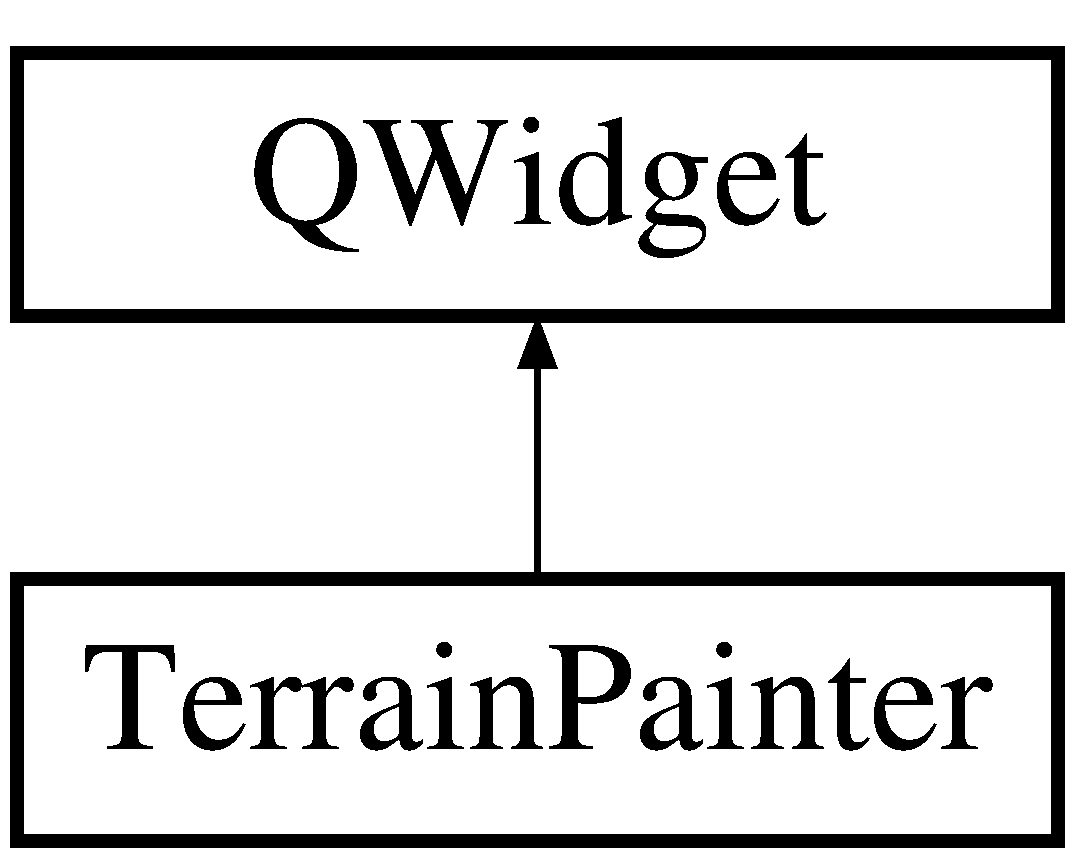
\includegraphics[height=2.000000cm]{class_terrain_painter}
\end{center}
\end{figure}
\subsection*{Public Member Functions}
\begin{DoxyCompactItemize}
\item 
\hyperlink{class_terrain_painter_a47946a56086bd611200820eb77ca3147}{Terrain\-Painter} (Q\-Widget $\ast$parent=0)
\begin{DoxyCompactList}\small\item\em Es el contructor por defecto. \end{DoxyCompactList}\item 
void \hyperlink{class_terrain_painter_a13d85e3171b965bd6e8f36fe1202e1c6}{set\-Map\-Maker} (\hyperlink{class_map_maker}{Map\-Maker} $\ast$p\-Map\-Maker)
\begin{DoxyCompactList}\small\item\em Es el metodo que se encarga de setear el creador de mapas. \end{DoxyCompactList}\item 
\hyperlink{class_updater}{Updater} $\ast$ \hyperlink{class_terrain_painter_a380f07447ee0f57907853d8e076d2b13}{updater} () const 
\begin{DoxyCompactList}\small\item\em Es el qthread que se encarga llamar al metodo de pintado del mapa. \end{DoxyCompactList}\item 
void \hyperlink{class_terrain_painter_adb52ca609c562dcfdfee84e844f7a32a}{set\-Updater} (\hyperlink{class_updater}{Updater} $\ast$\hyperlink{class_terrain_painter_a380f07447ee0f57907853d8e076d2b13}{updater})
\begin{DoxyCompactList}\small\item\em Setea el qthread. \end{DoxyCompactList}\item 
\hypertarget{class_terrain_painter_adb9dab4b8fe180bab8a722d7223a1048}{void \hyperlink{class_terrain_painter_adb9dab4b8fe180bab8a722d7223a1048}{unactivate\-Updater} ()}\label{class_terrain_painter_adb9dab4b8fe180bab8a722d7223a1048}

\begin{DoxyCompactList}\small\item\em se encarga de desactivar el qthread \end{DoxyCompactList}\item 
void \hyperlink{class_terrain_painter_a92d6e3c8f53f4f0a2ef6e896480d7080}{save\-Map} (Q\-String p\-Path, Q\-String p\-Name\-Of\-Map)
\begin{DoxyCompactList}\small\item\em Se encarga de guardar el mapa en xml. \end{DoxyCompactList}\item 
void \hyperlink{class_terrain_painter_aec8ab73fffb4c09518dab3544ce2812e}{load\-Map} (Q\-String p\-Path)
\begin{DoxyCompactList}\small\item\em Se encarga de cargar un mapa, si el archivo es invalido se arrojara un dialogo que indique el problema con el archivo. \end{DoxyCompactList}\item 
void \hyperlink{class_terrain_painter_aacd640eb9007ff64b3f82421f9bf57e6}{new\-Matrix} (int width, int height)
\begin{DoxyCompactList}\small\item\em Crea una matriz nueva intercambiandola con la anterior. \end{DoxyCompactList}\item 
\hypertarget{class_terrain_painter_addc5c0a796059d54c972b135228bb504}{virtual \hyperlink{class_terrain_painter_addc5c0a796059d54c972b135228bb504}{$\sim$\-Terrain\-Painter} ()}\label{class_terrain_painter_addc5c0a796059d54c972b135228bb504}

\begin{DoxyCompactList}\small\item\em Es el destructor. \end{DoxyCompactList}\item 
Q\-String \hyperlink{class_terrain_painter_ab7332903ffc7d966f34d033f42c29aee}{map\-Name} () const 
\begin{DoxyCompactList}\small\item\em Retorna el nombre representativo del mapa. \end{DoxyCompactList}\item 
void \hyperlink{class_terrain_painter_afb7f32fd9a50bb1f4845860bba8da920}{set\-Map\-Name} (const Q\-String \&\hyperlink{class_terrain_painter_ab7332903ffc7d966f34d033f42c29aee}{map\-Name})
\begin{DoxyCompactList}\small\item\em Setea el nombre representativo del mapa. \end{DoxyCompactList}\end{DoxyCompactItemize}
\subsection*{Protected Member Functions}
\begin{DoxyCompactItemize}
\item 
void \hyperlink{class_terrain_painter_a7d7e2b12bea08e85c6bae73fb6490fc1}{paint\-Event} (Q\-Paint\-Event $\ast$)
\begin{DoxyCompactList}\small\item\em Se encarga de printar el mapa. \end{DoxyCompactList}\item 
void \hyperlink{class_terrain_painter_ac9cd048e8cf4f027f72fbdfef1366587}{mouse\-Press\-Event} (Q\-Mouse\-Event $\ast$)
\begin{DoxyCompactList}\small\item\em Se encarga de gestionar los eventos de mouse del tipo presionar. \end{DoxyCompactList}\item 
void \hyperlink{class_terrain_painter_a27691132e68fc91464eb87b7572958ec}{mouse\-Release\-Event} (Q\-Mouse\-Event $\ast$)
\begin{DoxyCompactList}\small\item\em Es el metodo que se encarga de gestionar los eventos de mouse del tipo soltar. \end{DoxyCompactList}\item 
void \hyperlink{class_terrain_painter_aee20f0d6985434efc6a1b2c0d1af3fc0}{mouse\-Move\-Event} (Q\-Mouse\-Event $\ast$)
\begin{DoxyCompactList}\small\item\em Es el metodo que se encarga de gestionar los eventos demouse del tipo mover. \end{DoxyCompactList}\end{DoxyCompactItemize}


\subsection{Detailed Description}
Clase \hyperlink{class_terrain_painter}{Terrain\-Painter}, se encarga de pintar el mapa y gestionarlo asi como de guardarlo o cargar un mapa de un disco rigido. 

\subsection{Constructor \& Destructor Documentation}
\hypertarget{class_terrain_painter_a47946a56086bd611200820eb77ca3147}{\index{Terrain\-Painter@{Terrain\-Painter}!Terrain\-Painter@{Terrain\-Painter}}
\index{Terrain\-Painter@{Terrain\-Painter}!TerrainPainter@{Terrain\-Painter}}
\subsubsection[{Terrain\-Painter}]{\setlength{\rightskip}{0pt plus 5cm}Terrain\-Painter\-::\-Terrain\-Painter (
\begin{DoxyParamCaption}
\item[{Q\-Widget $\ast$}]{parent = {\ttfamily 0}}
\end{DoxyParamCaption}
)\hspace{0.3cm}{\ttfamily [explicit]}}}\label{class_terrain_painter_a47946a56086bd611200820eb77ca3147}


Es el contructor por defecto. 


\begin{DoxyParams}{Parameters}
{\em parent} & \\
\hline
\end{DoxyParams}


\subsection{Member Function Documentation}
\hypertarget{class_terrain_painter_aec8ab73fffb4c09518dab3544ce2812e}{\index{Terrain\-Painter@{Terrain\-Painter}!load\-Map@{load\-Map}}
\index{load\-Map@{load\-Map}!TerrainPainter@{Terrain\-Painter}}
\subsubsection[{load\-Map}]{\setlength{\rightskip}{0pt plus 5cm}void Terrain\-Painter\-::load\-Map (
\begin{DoxyParamCaption}
\item[{Q\-String}]{p\-Path}
\end{DoxyParamCaption}
)}}\label{class_terrain_painter_aec8ab73fffb4c09518dab3544ce2812e}


Se encarga de cargar un mapa, si el archivo es invalido se arrojara un dialogo que indique el problema con el archivo. 


\begin{DoxyParams}{Parameters}
{\em p\-Path} & es la direccion del archivo a cargar \\
\hline
\end{DoxyParams}
\hypertarget{class_terrain_painter_ab7332903ffc7d966f34d033f42c29aee}{\index{Terrain\-Painter@{Terrain\-Painter}!map\-Name@{map\-Name}}
\index{map\-Name@{map\-Name}!TerrainPainter@{Terrain\-Painter}}
\subsubsection[{map\-Name}]{\setlength{\rightskip}{0pt plus 5cm}Q\-String Terrain\-Painter\-::map\-Name (
\begin{DoxyParamCaption}
{}
\end{DoxyParamCaption}
) const}}\label{class_terrain_painter_ab7332903ffc7d966f34d033f42c29aee}


Retorna el nombre representativo del mapa. 

\begin{DoxyReturn}{Returns}
El nombre representativo del mapa 
\end{DoxyReturn}
\hypertarget{class_terrain_painter_aee20f0d6985434efc6a1b2c0d1af3fc0}{\index{Terrain\-Painter@{Terrain\-Painter}!mouse\-Move\-Event@{mouse\-Move\-Event}}
\index{mouse\-Move\-Event@{mouse\-Move\-Event}!TerrainPainter@{Terrain\-Painter}}
\subsubsection[{mouse\-Move\-Event}]{\setlength{\rightskip}{0pt plus 5cm}void Terrain\-Painter\-::mouse\-Move\-Event (
\begin{DoxyParamCaption}
\item[{Q\-Mouse\-Event $\ast$}]{e}
\end{DoxyParamCaption}
)\hspace{0.3cm}{\ttfamily [protected]}}}\label{class_terrain_painter_aee20f0d6985434efc6a1b2c0d1af3fc0}


Es el metodo que se encarga de gestionar los eventos demouse del tipo mover. 


\begin{DoxyParams}{Parameters}
{\em Mouse\-Event} & Es el evento \\
\hline
\end{DoxyParams}
\hypertarget{class_terrain_painter_ac9cd048e8cf4f027f72fbdfef1366587}{\index{Terrain\-Painter@{Terrain\-Painter}!mouse\-Press\-Event@{mouse\-Press\-Event}}
\index{mouse\-Press\-Event@{mouse\-Press\-Event}!TerrainPainter@{Terrain\-Painter}}
\subsubsection[{mouse\-Press\-Event}]{\setlength{\rightskip}{0pt plus 5cm}void Terrain\-Painter\-::mouse\-Press\-Event (
\begin{DoxyParamCaption}
\item[{Q\-Mouse\-Event $\ast$}]{m}
\end{DoxyParamCaption}
)\hspace{0.3cm}{\ttfamily [protected]}}}\label{class_terrain_painter_ac9cd048e8cf4f027f72fbdfef1366587}


Se encarga de gestionar los eventos de mouse del tipo presionar. 


\begin{DoxyParams}{Parameters}
{\em Mouse\-Event} & Es el evento \\
\hline
\end{DoxyParams}
\hypertarget{class_terrain_painter_a27691132e68fc91464eb87b7572958ec}{\index{Terrain\-Painter@{Terrain\-Painter}!mouse\-Release\-Event@{mouse\-Release\-Event}}
\index{mouse\-Release\-Event@{mouse\-Release\-Event}!TerrainPainter@{Terrain\-Painter}}
\subsubsection[{mouse\-Release\-Event}]{\setlength{\rightskip}{0pt plus 5cm}void Terrain\-Painter\-::mouse\-Release\-Event (
\begin{DoxyParamCaption}
\item[{Q\-Mouse\-Event $\ast$}]{}
\end{DoxyParamCaption}
)\hspace{0.3cm}{\ttfamily [protected]}}}\label{class_terrain_painter_a27691132e68fc91464eb87b7572958ec}


Es el metodo que se encarga de gestionar los eventos de mouse del tipo soltar. 


\begin{DoxyParams}{Parameters}
{\em Mouse\-Event} & Es el evento \\
\hline
\end{DoxyParams}
\hypertarget{class_terrain_painter_aacd640eb9007ff64b3f82421f9bf57e6}{\index{Terrain\-Painter@{Terrain\-Painter}!new\-Matrix@{new\-Matrix}}
\index{new\-Matrix@{new\-Matrix}!TerrainPainter@{Terrain\-Painter}}
\subsubsection[{new\-Matrix}]{\setlength{\rightskip}{0pt plus 5cm}void Terrain\-Painter\-::new\-Matrix (
\begin{DoxyParamCaption}
\item[{int}]{width, }
\item[{int}]{height}
\end{DoxyParamCaption}
)}}\label{class_terrain_painter_aacd640eb9007ff64b3f82421f9bf57e6}


Crea una matriz nueva intercambiandola con la anterior. 


\begin{DoxyParams}{Parameters}
{\em width} & es la cantidad de columnas deseadas, cada columna representa un conjunto de celdas \\
\hline
{\em height} & es la cantidad filas deseadas, cada fila representa un conjunto de celdas \\
\hline
\end{DoxyParams}
\hypertarget{class_terrain_painter_a7d7e2b12bea08e85c6bae73fb6490fc1}{\index{Terrain\-Painter@{Terrain\-Painter}!paint\-Event@{paint\-Event}}
\index{paint\-Event@{paint\-Event}!TerrainPainter@{Terrain\-Painter}}
\subsubsection[{paint\-Event}]{\setlength{\rightskip}{0pt plus 5cm}void Terrain\-Painter\-::paint\-Event (
\begin{DoxyParamCaption}
\item[{Q\-Paint\-Event $\ast$}]{}
\end{DoxyParamCaption}
)\hspace{0.3cm}{\ttfamily [protected]}}}\label{class_terrain_painter_a7d7e2b12bea08e85c6bae73fb6490fc1}


Se encarga de printar el mapa. 


\begin{DoxyParams}{Parameters}
{\em } & \\
\hline
\end{DoxyParams}
\hypertarget{class_terrain_painter_a92d6e3c8f53f4f0a2ef6e896480d7080}{\index{Terrain\-Painter@{Terrain\-Painter}!save\-Map@{save\-Map}}
\index{save\-Map@{save\-Map}!TerrainPainter@{Terrain\-Painter}}
\subsubsection[{save\-Map}]{\setlength{\rightskip}{0pt plus 5cm}void Terrain\-Painter\-::save\-Map (
\begin{DoxyParamCaption}
\item[{Q\-String}]{p\-Path, }
\item[{Q\-String}]{p\-Name\-Of\-Map}
\end{DoxyParamCaption}
)}}\label{class_terrain_painter_a92d6e3c8f53f4f0a2ef6e896480d7080}


Se encarga de guardar el mapa en xml. 


\begin{DoxyParams}{Parameters}
{\em name} & es el nombre representativo del mapa \\
\hline
{\em p\-Path} & es la direccion en la que se guardara el mapa \\
\hline
\end{DoxyParams}
\hypertarget{class_terrain_painter_a13d85e3171b965bd6e8f36fe1202e1c6}{\index{Terrain\-Painter@{Terrain\-Painter}!set\-Map\-Maker@{set\-Map\-Maker}}
\index{set\-Map\-Maker@{set\-Map\-Maker}!TerrainPainter@{Terrain\-Painter}}
\subsubsection[{set\-Map\-Maker}]{\setlength{\rightskip}{0pt plus 5cm}void Terrain\-Painter\-::set\-Map\-Maker (
\begin{DoxyParamCaption}
\item[{{\bf Map\-Maker} $\ast$}]{p\-Map\-Maker}
\end{DoxyParamCaption}
)}}\label{class_terrain_painter_a13d85e3171b965bd6e8f36fe1202e1c6}


Es el metodo que se encarga de setear el creador de mapas. 


\begin{DoxyParams}{Parameters}
{\em p\-Map\-Maker} & Es el creado de mapa \\
\hline
\end{DoxyParams}
\hypertarget{class_terrain_painter_afb7f32fd9a50bb1f4845860bba8da920}{\index{Terrain\-Painter@{Terrain\-Painter}!set\-Map\-Name@{set\-Map\-Name}}
\index{set\-Map\-Name@{set\-Map\-Name}!TerrainPainter@{Terrain\-Painter}}
\subsubsection[{set\-Map\-Name}]{\setlength{\rightskip}{0pt plus 5cm}void Terrain\-Painter\-::set\-Map\-Name (
\begin{DoxyParamCaption}
\item[{const Q\-String \&}]{map\-Name}
\end{DoxyParamCaption}
)}}\label{class_terrain_painter_afb7f32fd9a50bb1f4845860bba8da920}


Setea el nombre representativo del mapa. 


\begin{DoxyParams}{Parameters}
{\em map\-Name} & \\
\hline
\end{DoxyParams}
\hypertarget{class_terrain_painter_adb52ca609c562dcfdfee84e844f7a32a}{\index{Terrain\-Painter@{Terrain\-Painter}!set\-Updater@{set\-Updater}}
\index{set\-Updater@{set\-Updater}!TerrainPainter@{Terrain\-Painter}}
\subsubsection[{set\-Updater}]{\setlength{\rightskip}{0pt plus 5cm}void Terrain\-Painter\-::set\-Updater (
\begin{DoxyParamCaption}
\item[{{\bf Updater} $\ast$}]{updater}
\end{DoxyParamCaption}
)}}\label{class_terrain_painter_adb52ca609c562dcfdfee84e844f7a32a}


Setea el qthread. 


\begin{DoxyParams}{Parameters}
{\em updater} & es el qthread a utilizar \\
\hline
\end{DoxyParams}
\hypertarget{class_terrain_painter_a380f07447ee0f57907853d8e076d2b13}{\index{Terrain\-Painter@{Terrain\-Painter}!updater@{updater}}
\index{updater@{updater}!TerrainPainter@{Terrain\-Painter}}
\subsubsection[{updater}]{\setlength{\rightskip}{0pt plus 5cm}{\bf Updater} $\ast$ Terrain\-Painter\-::updater (
\begin{DoxyParamCaption}
{}
\end{DoxyParamCaption}
) const}}\label{class_terrain_painter_a380f07447ee0f57907853d8e076d2b13}


Es el qthread que se encarga llamar al metodo de pintado del mapa. 

\begin{DoxyReturn}{Returns}
el qthread que se encarga de actualizar 
\end{DoxyReturn}


The documentation for this class was generated from the following files\-:\begin{DoxyCompactItemize}
\item 
/home/cristianfernando/\-Documentos/git/\-Midgard\-Map\-Maker/terrainpainter.\-h\item 
/home/cristianfernando/\-Documentos/git/\-Midgard\-Map\-Maker/terrainpainter.\-cpp\end{DoxyCompactItemize}

\hypertarget{class_updater}{\section{Updater Class Reference}
\label{class_updater}\index{Updater@{Updater}}
}
Inheritance diagram for Updater\-:\begin{figure}[H]
\begin{center}
\leavevmode
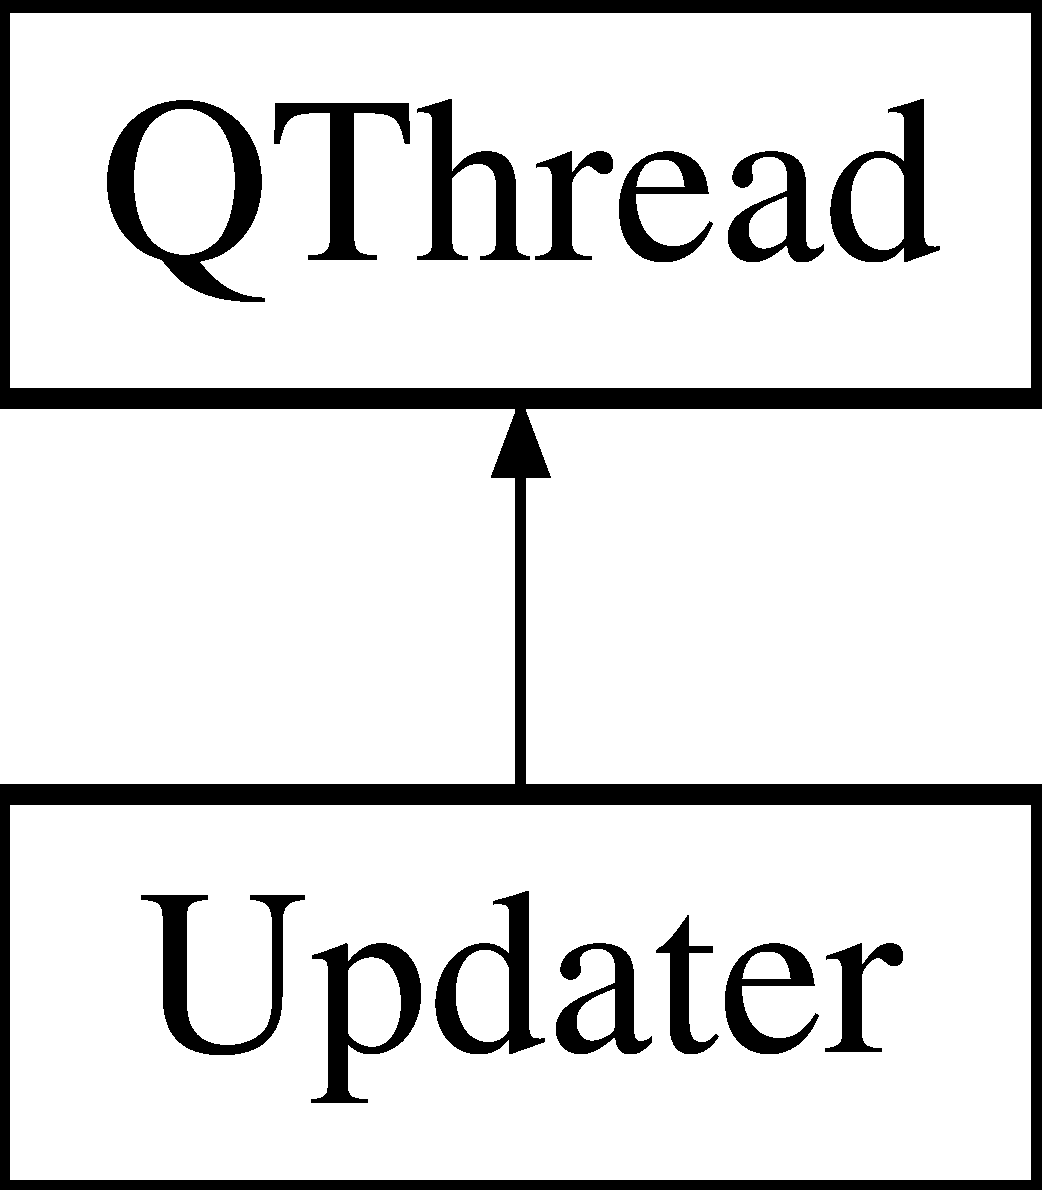
\includegraphics[height=2.000000cm]{class_updater}
\end{center}
\end{figure}
\subsection*{Signals}
\begin{DoxyCompactItemize}
\item 
\hypertarget{class_updater_a812f33261822358f982fbb932a3de65d}{void {\bfseries update} ()}\label{class_updater_a812f33261822358f982fbb932a3de65d}

\end{DoxyCompactItemize}
\subsection*{Public Member Functions}
\begin{DoxyCompactItemize}
\item 
\hypertarget{class_updater_adb60a473bc174de0ee06ee09c814e1a2}{{\bfseries Updater} (Q\-Object $\ast$parent=0)}\label{class_updater_adb60a473bc174de0ee06ee09c814e1a2}

\item 
\hypertarget{class_updater_abd76987a878910ff4687cac6cd63859d}{void {\bfseries run} ()}\label{class_updater_abd76987a878910ff4687cac6cd63859d}

\item 
\hypertarget{class_updater_a1bf91b5b0d6a3d3edd7da8ede14f5746}{void {\bfseries stop} ()}\label{class_updater_a1bf91b5b0d6a3d3edd7da8ede14f5746}

\end{DoxyCompactItemize}


The documentation for this class was generated from the following files\-:\begin{DoxyCompactItemize}
\item 
/home/cristianfernando/\-Documentos/git/\-Midgard\-Map\-Maker/updater.\-h\item 
/home/cristianfernando/\-Documentos/git/\-Midgard\-Map\-Maker/updater.\-cpp\end{DoxyCompactItemize}

%--- End generated contents ---

% Index
\newpage
\phantomsection
\addcontentsline{toc}{chapter}{Index}
\printindex

\end{document}
